\documentclass{beamer}
\usepackage{graphicx}
\graphicspath{ {./images/} }

\usepackage[utf8]{inputenc}


%Information to be included in the title page:
\title{Myo Armband Virtual Keyboard}
\author{Judah Zammit}

\begin{document}

\frame{\titlepage}

\AtBeginSection[]{
  \begin{frame}
  \vfill
  \centering
  \begin{beamercolorbox}[sep=8pt,center,shadow=true,rounded=true]{title}
    \usebeamerfont{title}\insertsectionhead\par%
  \end{beamercolorbox}
  \vfill
  \end{frame}
}

\section{Data Splitting}
\begin{frame}
\frametitle{Gyroscope X-Axis}
\begin{figure}
	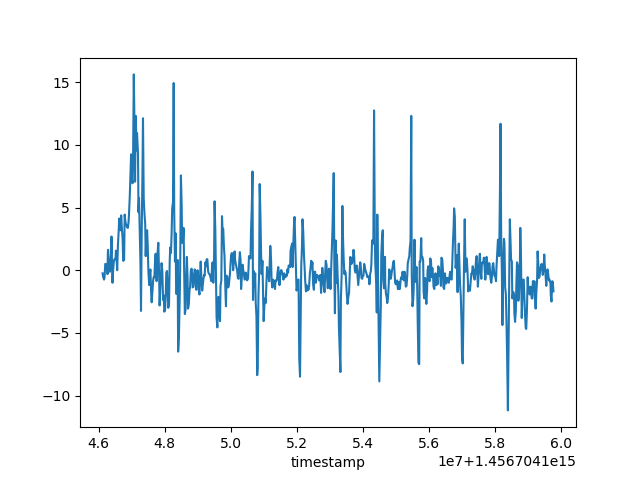
\includegraphics[scale=.70]{vanilla_gyro}
\end{figure}
\end{frame}

\begin{frame}
\frametitle{Mean Absolute Deviation}
\begin{figure}
	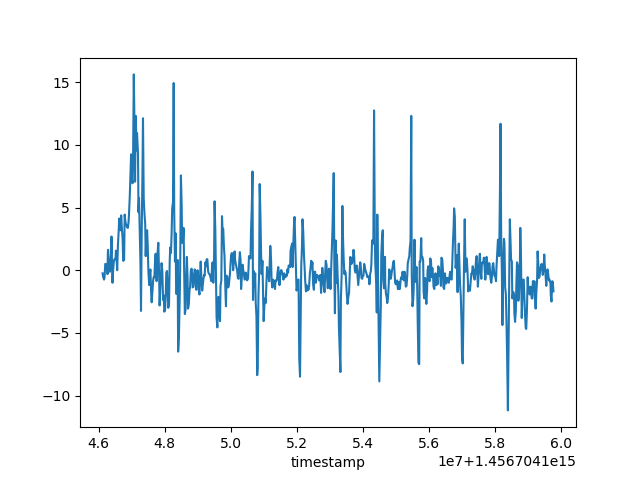
\includegraphics[scale=.35]{vanilla_gyro}
	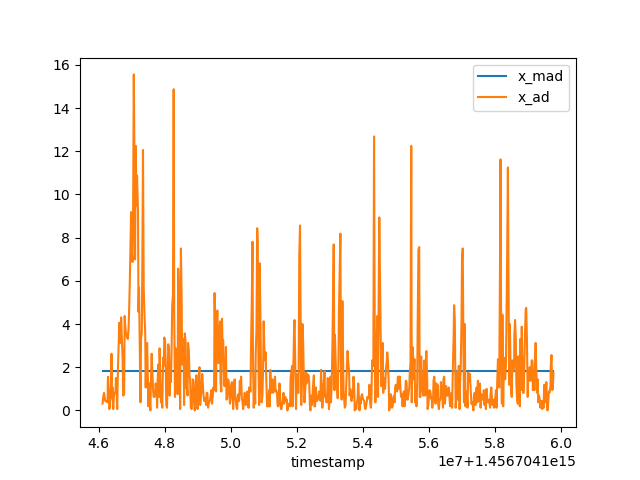
\includegraphics[scale=.35]{mad_ad}
\end{figure}
\end{frame}

\begin{frame}
\frametitle{Windowed Mean Absolute Deviation}
\begin{figure}
	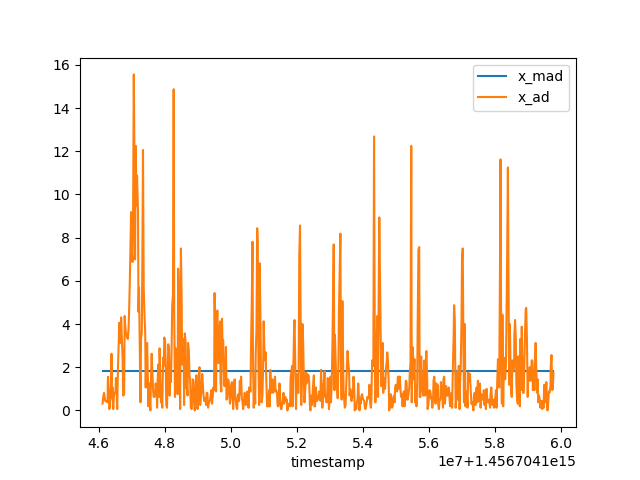
\includegraphics[scale=.35]{mad_ad}
	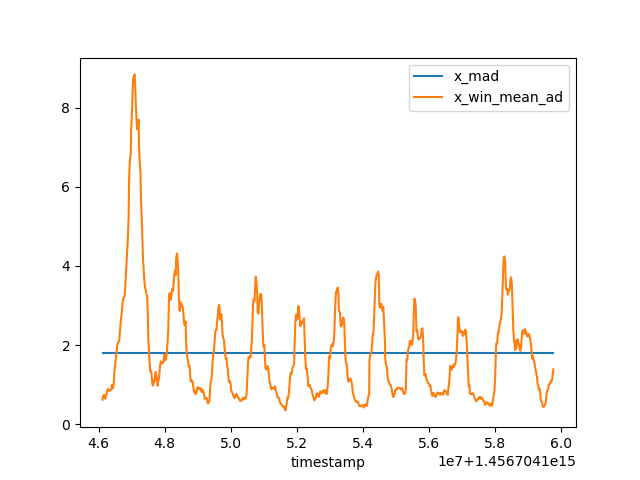
\includegraphics[scale=.35]{mad_win_ad}
\end{figure}

\end{frame}
\begin{frame}
\frametitle{Activity}
\begin{figure}
	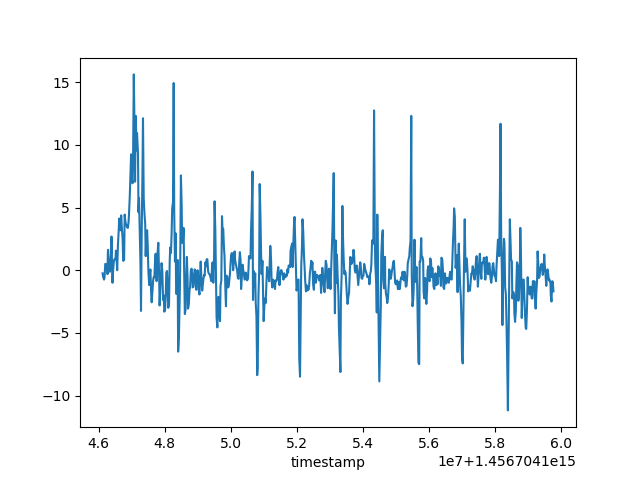
\includegraphics[scale=.35]{vanilla_gyro}
	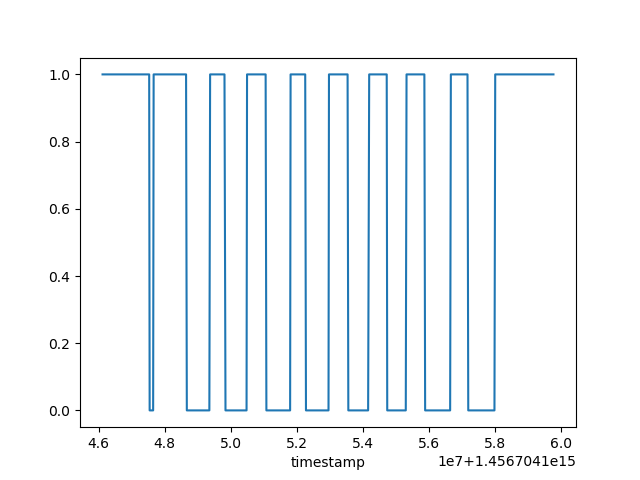
\includegraphics[scale=.35]{activity}
\end{figure}


\end{frame}

\begin{frame}

\frametitle{Split Points}

\begin{figure}
	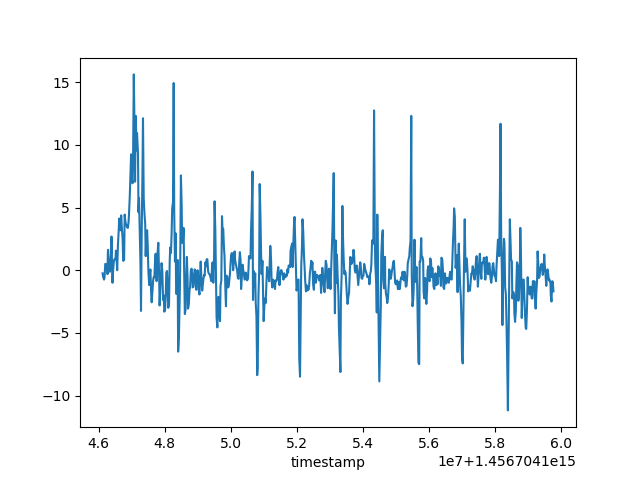
\includegraphics[scale=.15]{vanilla_gyro}
\end{figure}

\begin{figure}
	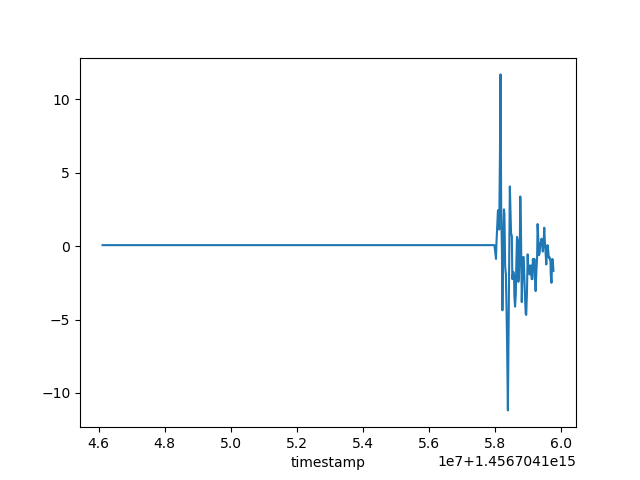
\includegraphics[scale=.15]{point_1}
    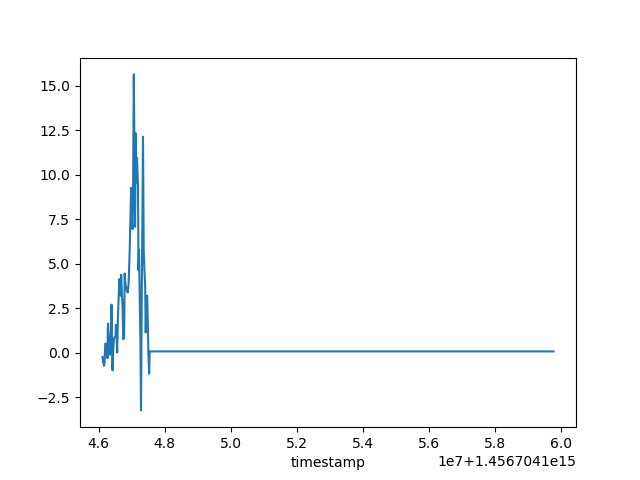
\includegraphics[scale=.15]{point_2}
    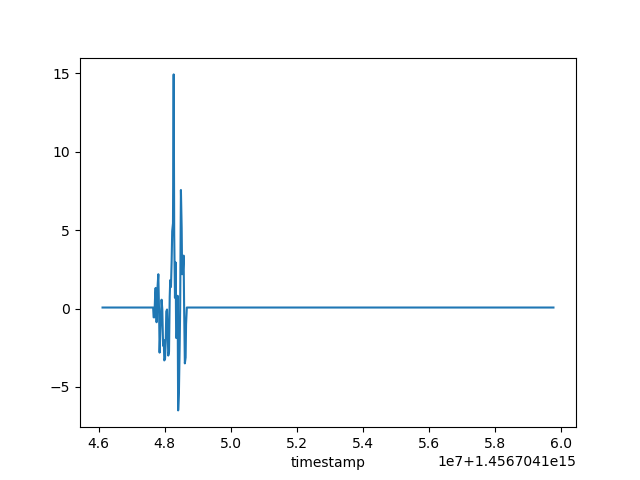
\includegraphics[scale=.15]{point_3}
    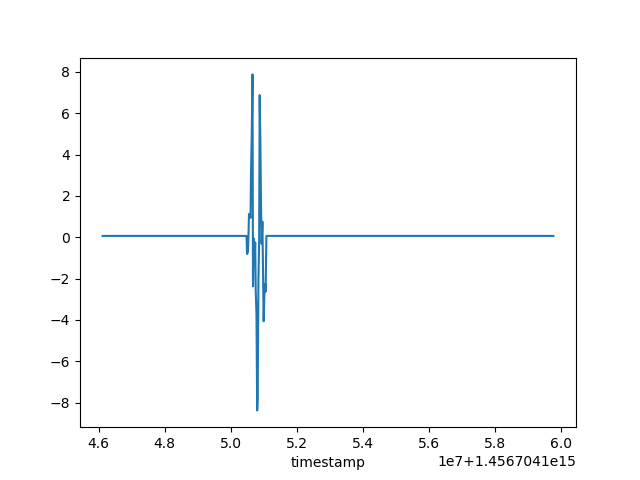
\includegraphics[scale=.15]{point_4}
\end{figure}

\begin{figure}
	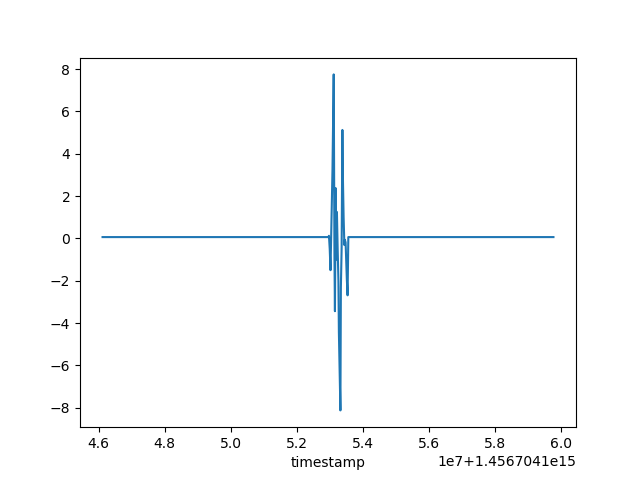
\includegraphics[scale=.15]{point_5}
    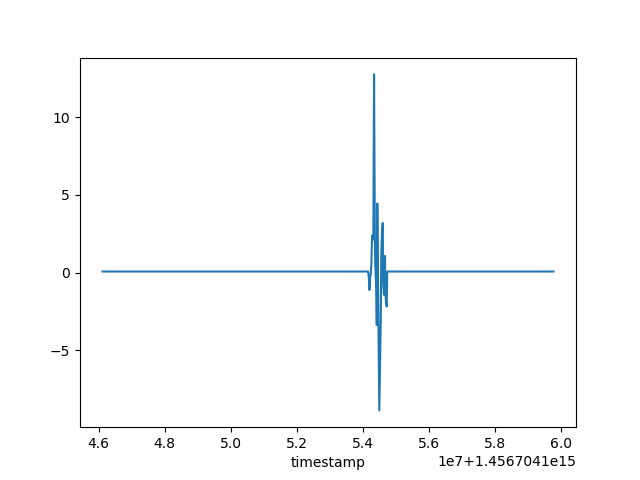
\includegraphics[scale=.15]{point_6}
    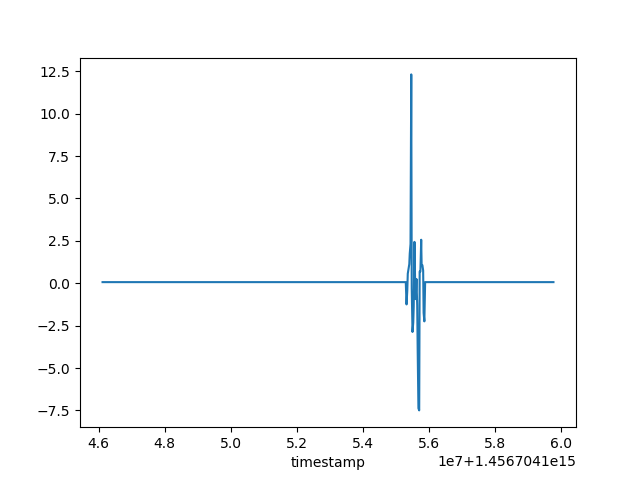
\includegraphics[scale=.15]{point_7}
\end{figure}


\begin{figure}
	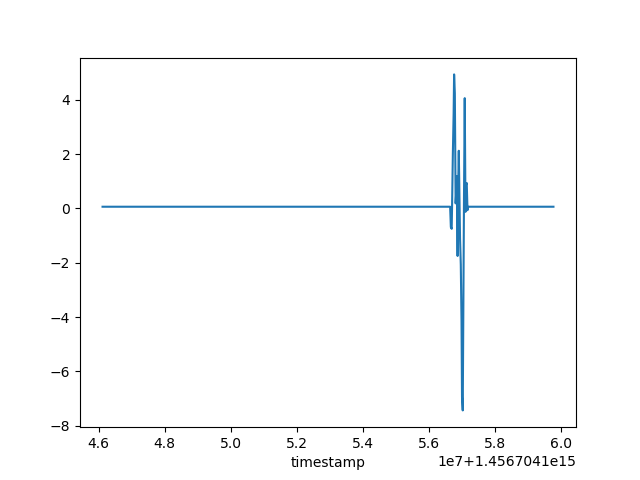
\includegraphics[scale=.15]{point_8}
    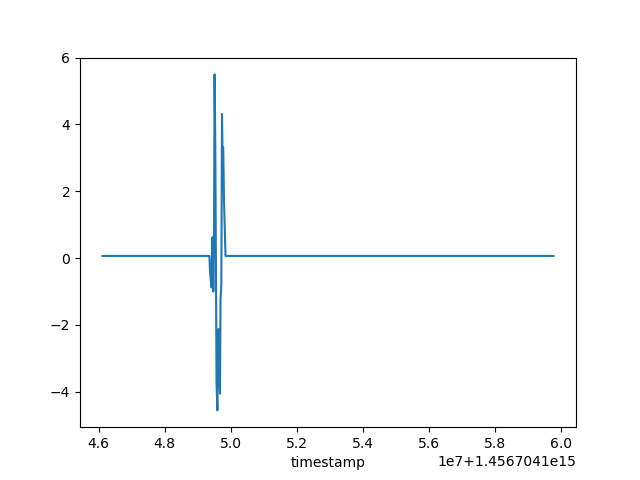
\includegraphics[scale=.15]{point_9}
    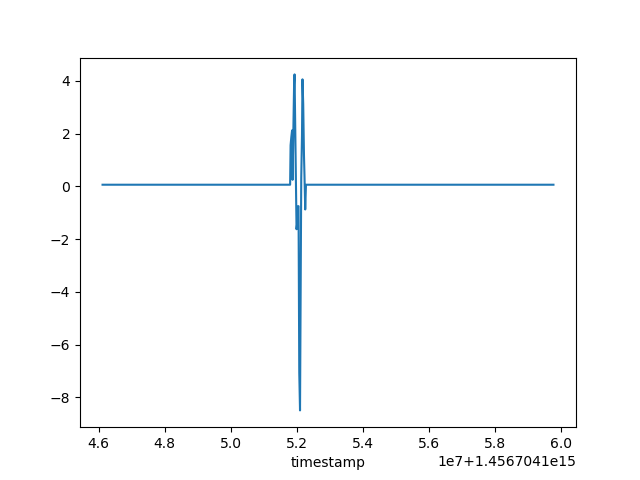
\includegraphics[scale=.15]{point_10}
\end{figure}

\end{frame}

\section{Feature Extraction}
\begin{frame}
\frametitle{Physical Data Feature Extraction}
We use the following statistics as features:
\begin{itemize}
\item $Median$
\item $Mean\, Absolute\, Deviation = \frac{\sum_{i = 1}^{N} |x_i - \mu|}{N}$
\item $Magnitude = \frac{\sum_{i = 1}^{N}\sqrt{x_i^2 + y_i^2 + z_i^2}}{N}$
\end{itemize}
\end{frame}
\begin{frame}

\begin{figure}
	
\includegraphics[scale=.35]{phys_fe}
\end{figure}

\end{frame}

\begin{frame}
\frametitle{EMG Data Feature Extraction}
We use the following statistics as features:
\begin{itemize}
\item $Variance = \frac{\sum_{i = 1}^{N}(x_i - \mu)^2}{N}$
\item $Mean\, Absolute\, Value = \frac{\sum_{i = 1}^{N} |x_i|}{N}$
\item $Waveform\,Length = \sum_{i = 1}^{N}|x_i - x_{i + 1}|$
\end{itemize}
\end{frame}

\begin{frame}

\begin{figure}
	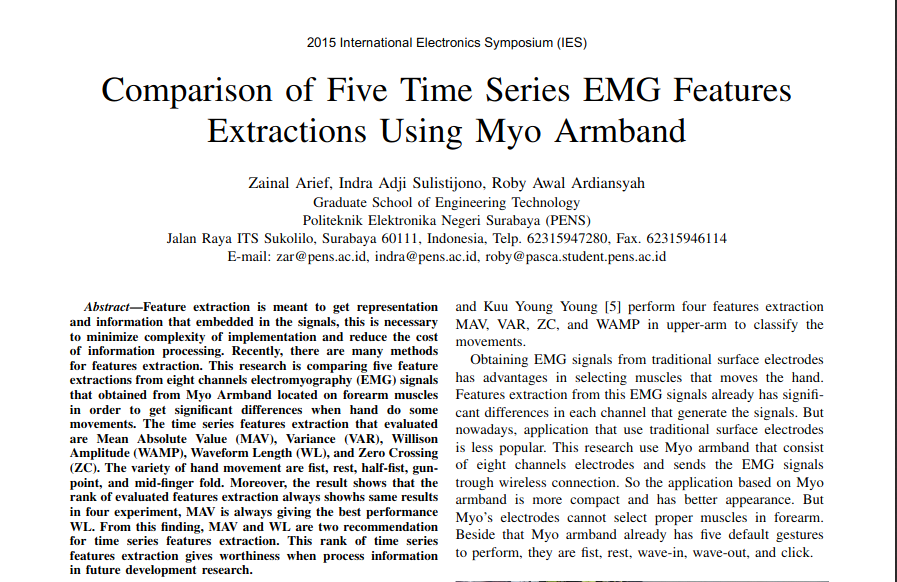
\includegraphics[scale=.35]{emg_fe}
\end{figure}

\end{frame}

\section{Results}

\begin{frame}
\frametitle{Results on Physical Data}


\begin{tabular}{ |p{2cm}|p{2cm}||p{2cm}|p{2cm}|  }
 \hline
 &CV-Accuracy & Train-Accuracy & Test-Accuracy \\
 \hline
 Tree & 91\% & 100\%  & 100\% \\
 \hline
 RF & 93\%    & 100\%   & 100\% \\
 \hline
 NN & 93\%   & 100\%  & 100\% \\
 \hline
\end{tabular}

\end{frame}

\begin{frame}
\frametitle{Results on EMG Data}

\begin{tabular}{ |p{2cm}|p{2cm}||p{2cm}|p{2cm}|  }
 \hline
 &CV-Accuracy & Train-Accuracy & Test-Accuracy \\
 \hline
 Tree & 62\% & 100\%  & 100\% \\
 \hline
 RF & 82\%    & 100\%   & 100\% \\
 \hline
 NN & 91\%   & 100\%  & 100\% \\
 \hline
\end{tabular}

\end{frame}

\begin{frame}
\frametitle{Results on Both EMG and Physical Data}

\begin{tabular}{ |p{2cm}|p{2cm}||p{2cm}|p{2cm}|  }
 \hline
 &CV-Accuracy & Train-Accuracy & Test-Accuracy \\
 \hline
 Tree & 89\% & 100\%  & 100\% \\
 \hline
 RF & 93\%    & 100\%   & 100\% \\
 \hline
 NN & 97\%   & 100\%  & 100\% \\
 \hline
\end{tabular}

\end{frame}

\begin{frame}
\frametitle{Decision Tree}
\begin{figure}
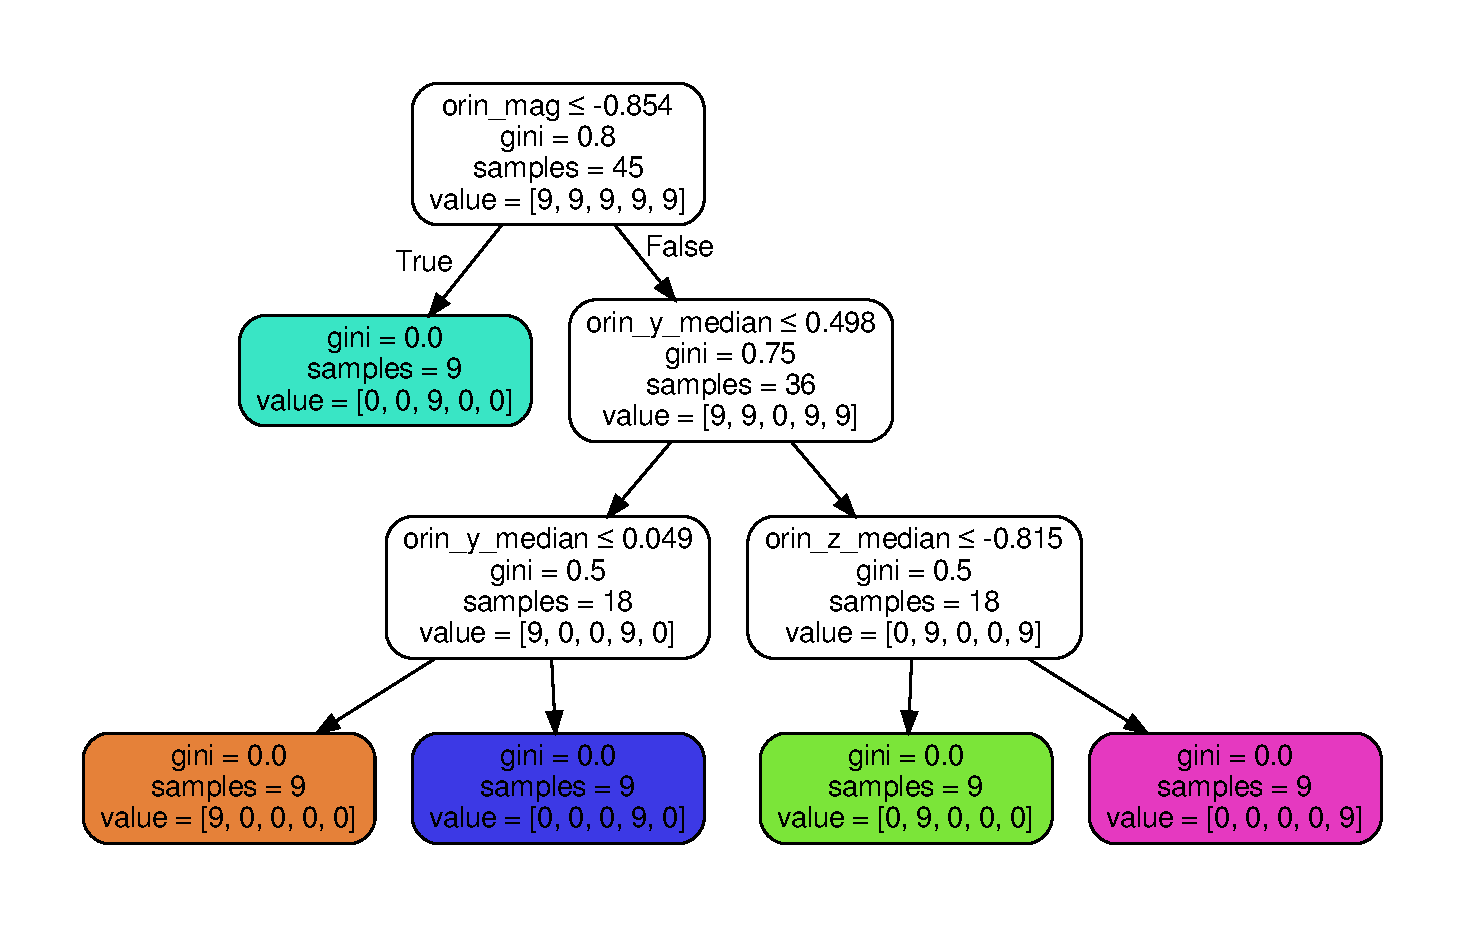
\includegraphics[scale=.3]{tree}
\end{figure}
\end{frame}


\end{document}